\documentclass[a4paper,14pt]{article}
\usepackage{graphicx}
\usepackage{booktabs}
\usepackage[margin=1in]{geometry}
\usepackage{amsmath}
\usepackage[labelfont=bf]{caption}

\usepackage{hyperref}
\usepackage{subcaption}
\usepackage{listings} 
\usepackage{setspace}  
\usepackage{color}
\usepackage{xcolor}
\usepackage{listings}
\usepackage{xepersian}

\settextfont{XB Yas}
\setlength\parindent{0pt}


\begin{document}
	\fontsize{14}{14}\selectfont
	
	
	
	\begin{titlepage}
		\begin{center}
			
			\Huge
			
			\textbf{پروژه Bonus درس ارزیابی کارایی سیستم های کامپیوتری فصل چهارم}
			
			\vspace{1cm}
			
			\LARGE
			
			
			نام استاد: دکتر احمد خونساری\\
				تاریخ: \today
			
			\vspace{1cm}
			
			
\includegraphics[width=0.5\textwidth]{Figures/teh.png}
			
			
			
			نویسندگان:\\
			
			\vspace{0.5cm}
			
			امیرحسین مهرورز: 810100484\\
			آرمان داوری: 810199153\\
			مجتبی مژگان فر: 810100471\\
			نیما شکری: 810199200\\
			یگانه کردی: 810100551\\
			هادی قوامی نژاد: 810100438\\
			مینا فریدی: 810100430\\
			فاروق شایسته رودی: 810199198\\
			محمدمهدی یادگاری فرد: 81099308
			
			\vspace{0.5cm}
			
		
		
			
		\end{center}
	\end{titlepage}
	
	\newpage
	
	
\section*{جواب سوال اول:}	
در این سوال ابتدا نمودار x را رسم می کنیم. به این طریق که به x آرایه ای با توزیع یکنواخت از 200 عدد بین 1 و 1- می دهیم و با mathplotlib رسم میکنیم. سپس Fy را بر حسب x می نویسیم یک بار برای قسمت a و یک بار قسمت b. خطوط آبی رنگ نشان دهنده x هستند و خطوط نارنجی Fy را نشان می دهند.  تابع pdf در واقع مشتق تابع Fy است که با نگاه کردن به نمودار می توان فرمول آن را بدست آورد.

کد مربوط به این سوال در زیر آمده است:\\

\fontsize{12}{12}\selectfont
\begin{latin}
	\begin{lstlisting}
		
import numpy as np
from matplotlib import pyplot as plt

if __name__ == '__main__':
  #a
  x = np.arange(-1,1,0.01)
  plt.figure(0)
  plt.plot(x)
  dx = np.arange(-100,100,1)
  Fy = np.absolute(x)
  Fy = np.power(Fy,0.5)
  plt.plot(Fy)
  plt.show()

  #b
  x = np.arange(-1,1,0.01)
  plt.figure(1)
  plt.plot(x)
  dx = np.arange(-100,100,1)
  Fy = np.absolute(x)
  Fy = -1* np.log(Fy)
  plt.plot(Fy)
  plt.show()
		
	\end{lstlisting}
\end{latin}
\fontsize{14}{14}\selectfont

همچنین تصویر خروجی کد بالا را در زیر مشاهده میکنیم:\\

\begin{center}
	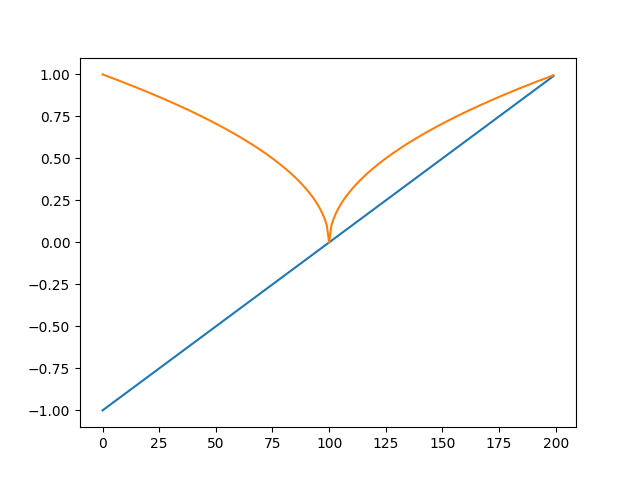
\includegraphics[width=0.5\textwidth]{Figures/fig_1.png}
\end{center}
\begin{center}
	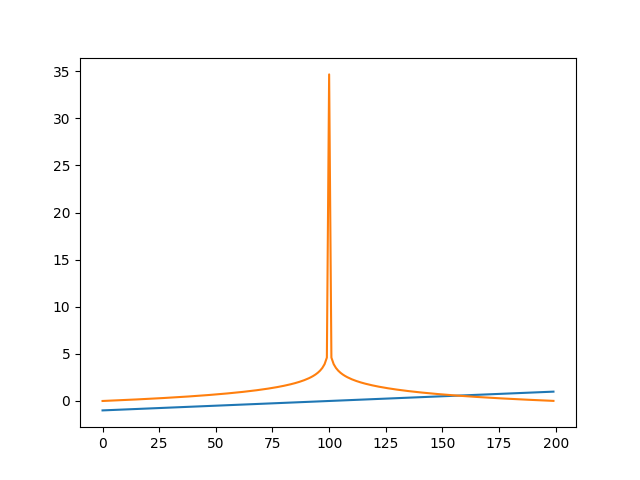
\includegraphics[width=0.5\textwidth]{Figures/fig_2.png}
\end{center}


\section*{جواب سوال پنجم:}	
دو متغیر تصادفی با توزیع یکنواخت x و y در بازه صفر و یک داریم و از هم مستقل هستند.
طبق محاسبات تابع توزیع تجمعی 
$|X-Y|$
برابر با
$1 - (1 - z)^2$
می باشد.

و  تابع چگالی احتمال برابر:
$$
f_z(z) =
\begin{cases}
	2(1 - z), & if \hspace{1mm} 0 \leq z \leq 1	, \\
	0, & otherwise.
\end{cases}
$$	

می باشد. موارد فوق الذکر در کد پیاده سازی شده است.\\

در زیر کد مربوط به پیاده سازی این سوال آمده است:\\

\fontsize{12}{12}\selectfont
\begin{latin}
	\begin{lstlisting}
		
print("The CDF of Z=|X-Y| is equal to : F(z) = 1-((1-z)*(1-z))")
print("The PDF of Z=|X-Y| is equal to : f(z) = 2*(1-z)")

z = float(input("Please Enter z : "))

CDF = PDF = 0

if (z >= 0 and z <= 1) :
  CDF = 1 - ((1-z)*(1-z))
  PDF = 2*(1-z)
elif z<0 :
  CDF = 0
  PDF = 0
else :
  CDF = 1
  PDF = 0

print("The CDF of Z=|X-Y| for z=" + str(z) + " is : " + str(CDF))
print("The PDF of Z=|X-Y| for z=" + str(z) + " is : " + str(PDF))
		
	\end{lstlisting}
\end{latin}
\fontsize{14}{14}\selectfont

نتیجه ی  خروجی به ازای z برابر با 2 به صورت زیر است:\\

\fontsize{12}{12}\selectfont
\begin{latin}
	\begin{lstlisting}
		
The CDF of Z=|X-Y| is equal to : F(z) = 1-((1-z)*(1-z))
The PDF of Z=|X-Y| is equal to : f(z) = 2*(1-z)
Please Enter z : 2
The CDF of Z=|X-Y| for z=2.0 is : 1
The PDF of Z=|X-Y| for z=2.0 is : 0
		
	\end{lstlisting}
\end{latin}
\fontsize{14}{14}\selectfont


\section*{جواب سوال نه:}
در این کد، پارامترهای توزیع های x و y و مقدار z اخذ می شود. سپس تابع چگالی احتمال و تابع توزیع تجمعی برای دوحالت و بر اساس اینکه z بزرگ تر مساوی 0 باشد و یا z کوچکتر از 0 باشد طبق حل ریاضی آن، محسابه می شود. در نهایت تابع توزیع Z بزرگ را نمایش می دهد.

\noindent input
پایانی به علت توانایی اجرا برنامه بدون IDE و با دابل کلیک نوشته شده است.

کد پیاده  سازی این سوال به صورت زیر میباشد:\\

\fontsize{12}{12}\selectfont
\begin{latin}
	\begin{lstlisting}
		
#! python3.9
# Q9.py
# Author : Pooya Jamshidi
# This code represent The result of Problem No. 9 in Section 4 
#of Bertsekas Book.
import math

lambda_param = float(input
  ("Please Enter The lambda parameter of variable X : "))
mu_param = float(input
  ("Please Enter The mu parameter of variable Y : "))
z = float(input("Please Enter z : "))

cdf = pdf = 0

if z >= 0:
  cdf = 1 - (mu_param * math.exp(-lambda_param * z)) /
     (mu_param + lambda_param)
  pdf = (lambda_param * mu_param * 
    math.exp(-lambda_param * z)) / (mu_param + lambda_param)
else:
  cdf = (lambda_param * math.exp(mu_param * z))
     / (mu_param + lambda_param)
  pdf = (lambda_param * mu_param * math.exp(mu_param * z))
     / (mu_param + lambda_param)

print("The CDF of Z=X-Y for z=" + str(z) + " is : " + str(cdf))
print("The PDF of Z=X-Y for z=" + str(z) + " is : " + str(pdf))

input("Thank You for your time, press Enter for exit... ")
		
	\end{lstlisting}
\end{latin}
\fontsize{14}{14}\selectfont

نتیجه ی حاصل از خروحی این کد به صورت زیر میباشد:\\


\fontsize{12}{12}\selectfont
\begin{latin}
	\begin{lstlisting}
		
Please Enter The lambda parameter of variable X : 1
Please Enter The mu parameter of variable Y : 2
Please Enter z : 3
The CDF of Z=X-Y for z=3.0 is : 0.9668086210880907
The PDF of Z=X-Y for z=3.0 is : 0.0331913789119093
		
	\end{lstlisting}
\end{latin}
\fontsize{14}{14}\selectfont


\section*{جواب سوال سیزده:}

در این  سوال از ما خواسته شده است تا ثابت کنیم که PDF های x+y و x-y با شیفت دیگری بدست می آیند. ابتدا توزیع نرمال مربوط به x و y را ایجاد و رسم میکنیم. با توجه به صوت سوال ابتدا شرطی قرار میدهیم تا اعداد خارج از بازه ی گفته شده یعنی a و b برابر با صفر شوند. سپس توزیع x+y و x-y را به کمک x و y به صورت جداگانه بدست می آوریم و رسم میکنیم. همانطور که در خروجی مشخص است، در پلات دیده میشود که این دو  شکل با شیفت نسبت به یکدیگر بدست آمده اند.\\

کد حل این سوال در زیر آمده است:\\

\fontsize{12}{12}\selectfont
\begin{latin}
	\begin{lstlisting}
		
import numpy as np
import matplotlib.pyplot as plt
a = 1
b = 10
mu, sigma = 5.5, 0.1 # mean and standard deviation
x = np.random.normal(mu, sigma, 1000)
y = np.random.normal(mu, sigma, 1000)

for i in range(len(x)):
  if x[i]<a:
    x[i]=0
  elif x[i]> b:
    x[i]=0

for i in range(len(y)):
  if y[i]<a:
    y[i]=0
  elif y[i]> b:
    y[i]=0
count, bins, ignored = plt.hist(x, 30, density=True)
plt.plot(bins, 1/(sigma * np.sqrt(2 * np.pi)) *
np.exp( - (bins - mu)**2 / (2 * sigma**2) ),
linewidth=2, color='r')
count, bins, ignored = plt.hist(y, 30, density=True)
plt.plot(bins, 1/(sigma * np.sqrt(2 * np.pi)) *
np.exp( - (bins - mu)**2 / (2 * sigma**2) ),
linewidth=2, color='b')
plt.show()

s = x + y
count, bins, ignored = plt.hist(s, 30, density=True)
plt.plot(bins, 1/(sigma * np.sqrt(2 * np.pi)) *
np.exp( - (bins - mu)**2 / (2 * sigma**2) ),
linewidth=2, color='r')
plt.show()

s = x - y
count, bins, ignored = plt.hist(s, 30, density=True)
plt.plot(bins, 1/(sigma * np.sqrt(2 * np.pi)) *
np.exp( - (bins - mu)**2 / (2 * sigma**2) ),
linewidth=2, color='r')
plt.show()
		
	\end{lstlisting}
\end{latin}
\fontsize{14}{14}\selectfont


نتیجه ی حاصل از خروجی این کد به صورت زیر است:\\

\begin{center}
	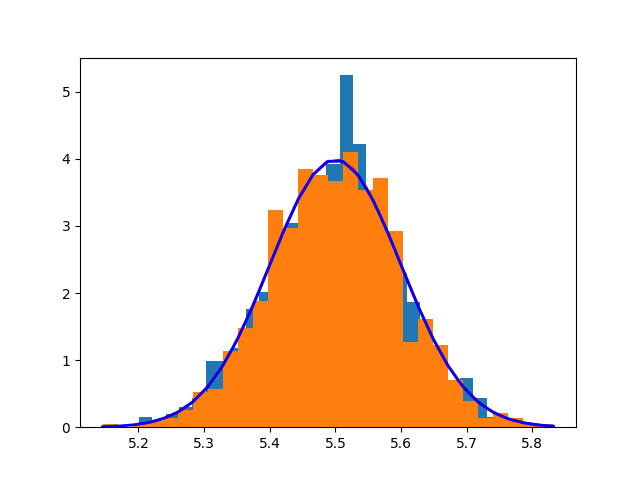
\includegraphics[width=0.5\textwidth]{Figures/fig_3.png}
\end{center}

\begin{center}
	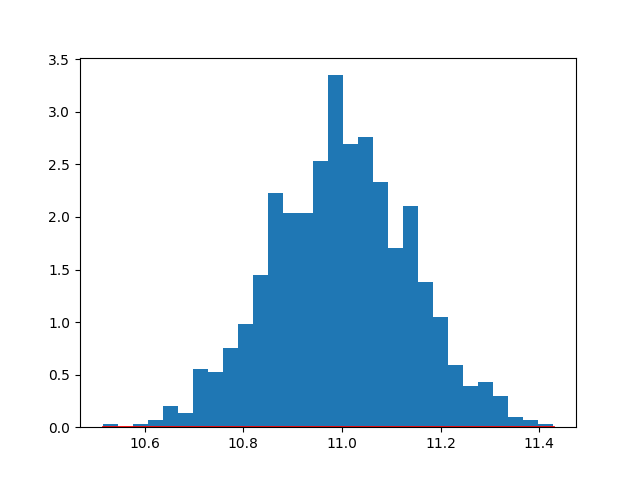
\includegraphics[width=0.5\textwidth]{Figures/fig_4.png}
\end{center}


\begin{center}
	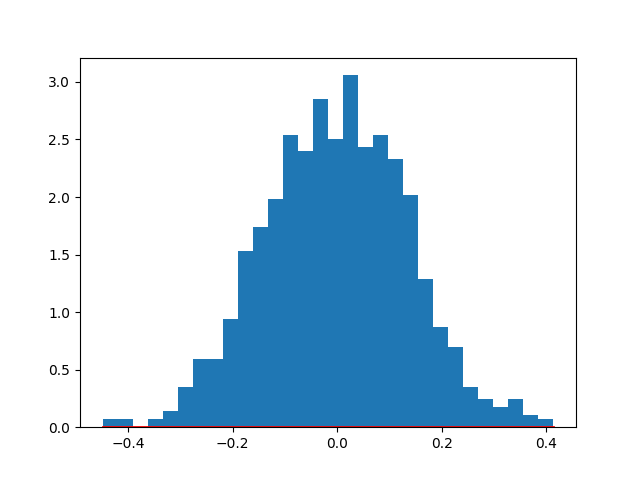
\includegraphics[width=0.5\textwidth]{Figures/fig_5.png}
\end{center}


\section*{جواب سوال هفده:}
در این کد می خواهیم ثابت کنیم،
$x+y$ 
و
$x-y$
ناهمبسته هستند.
برای ناهمبستگی بایستی
coefficient correlation 
شان صفر شود.

\noindent نخست چند المنتی بودن آرایه x اخذ می شود، سپس ورودی می دهیم. برای y نیز به همین صورت عمل نموده و واریانس x و y را محاسبه می کنیم.

اگر واریانس مساوی باشد ادامه می دهیم در غیر اینصورت می آید بیرون (در خط 13 کد).

اگر واریانس یکی باشد
$x+y$ 
و
$x-y$
را حساب نموده و از طریق تابع مندرج در خط 24، 
coefficient correlation 
را می دهد و اگر صفر باشد ناهمبسته هستند.

در آرایه sum ،
$x+y$
ها ریخته شده است و در آرایه sub ،
$x-y$
ها ریخته شده است.\\

کد مربوط به پیاده سازی این سوال به صورت زیر است:\\

\fontsize{12}{12}\selectfont
\begin{latin}
	\begin{lstlisting}
		
import numpy as np
if __name__ == '__main__':
  x = []
  n = int(input("Enter number of elements of x : "))
  for i in range(0, n):
    temp = int(input("enter x elements : "))
    x.append(temp)  # adding the element
  y = []
  n = int(input("Enter number of elements of y : "))
  for i in range(0, n):
    temp = int(input("enter y elements : "))
    y.append(temp)  # adding the element
  if np.var(x) == np.var(y):
    print("Two random variables have the same variance.")
    sum = []
    sub = []
    for i in x:
      for j in y:
        sum.append(i+j)
    for i in x:
      for j in y:
        sub.append(i-j)

    cor = np.corrcoef(sum, sub)
    if cor[0,1] == 0:
      print("The two random variables set 
        (X+Y) and (X-Y) are uncorrelated")
    else:
      print("(X+Y) and (X-Y) are Correlated")
  else:
    print("Two random variables DONT have the same variance.")
		
	\end{lstlisting}
\end{latin}
\fontsize{14}{14}\selectfont

\section*{جواب سوال بیست و نه:}
برای پیاده سازی فرمول 
$M(s)$
و محاسبه گشتاور های مرتبط با سیستم، ابتدا کتابخانه 
\lr{\textbf{sympy}}
را اضافه می کنیم. سپس برای محاسبه مشتق تابع 
\lr{calc\_derivative(n:int)$\rightarrow$ float}
را تعریف می کنیم. متغیر
$n$
دفعات مشتق گیری را مشخص
می نماییم.
با استفاده از دستور 
\lr{Symbol}
متغیر 
$s$
را به عنوان یک نماد تعریف می نماییم. پس از تعریف متغیر با توجه به رابطه محاسبه شده تابع مرتبط با 
$M(s)$
را پیاده سازی می کنیم:
$$
func_s=M(s)=\frac{1}{2}e^{s}+\frac{1}{4}e^{2*s}+\frac{1}{4}e^{3*s}
$$ 
در ادامه با استفاده از دستور 
\lr{func\_s.diff(s,n)}
عملیات مشتق گیری را انجام می دهیم و در متغیر 
\lr{func\_s\_derivative}
ذخیره می کنیم.
و با استفاده از دستور
\lr{func\_s\_derivative.subs(s,0)}
با قرار دادن
$s=0$
مقدار عددی مشتق محاسبه شده را محاسبه میکنیم.

با توجه به اینکه می خواهیم گشتاور های اول تا سوم را محاسبه کنیم تابع نوشته شده را در حلقه 
\lr{for}
نوشته شده قرار می دهیم و مقادیر خواسته شده را  در خروجی چاپ می کنیم.\\

کد مربوط به پیاده سازی این سوال در زیر آمده است:\\

\fontsize{12}{12}\selectfont
\begin{latin}
	\begin{lstlisting}
		
from sympy import *


def calc_derivative(n:int) -> float:
  """
  define S as a symbolic variable
  M(s) = (1/2)*exp(s)+(1/4)*exp(2*s)+(1/4)*exp(3*s)
  with derivative M(s) with respect to s
  we can calculate moments of distribution
  """
  s = Symbol('s')
  func_s = (1/2)*exp(s)+(1/4)*exp(2*s)+(1/4)*exp(3*s)
  func_s_derivative = func_s.diff(s,n)
  return func_s_derivative,func_s_derivative.subs(s,0)


for i in range(1,4):
  print("E[X^%d]=%s: for s=0 we have: 
    %.2f"%(i,calc_derivative(i)[0],calc_derivative(i)[1]))
		
	\end{lstlisting}
\end{latin}
\fontsize{14}{14}\selectfont

خروجی این کد به  صورت زیر میباشد:\\

\fontsize{12}{12}\selectfont
\begin{latin}
	\begin{lstlisting}
		
E[X^1]=0.75*exp(3*s) + 0.5*exp(2*s) + 0.5*exp(s): for s=0 we have: 1.75
E[X^2]=(2.25*exp(2*s) + 1.0*exp(s) + 0.5)*exp(s): for s=0 we have: 3.75
E[X^3]=(6.75*exp(2*s) + 2.0*exp(s) + 0.5)*exp(s): for s=0 we have: 9.25
		
	\end{lstlisting}
\end{latin}
\fontsize{14}{14}\selectfont

\section*{جواب سوال سی و سوم:}
در این کد برای به دست آوردن تابع چگالی احتمال از معکوس تبدیل داده شده در صورت سوال که تبدیل لاپلاس است، استفاده شده است.\\

کد این سوال در زیر آمده است:\\


\fontsize{12}{12}\selectfont
\begin{latin}
	\begin{lstlisting}
		
import sympy as sp
s, x = sp.symbols('s, x')
expression = (1/3 * 2/(2-s)) + (2/3 * 3/(3-s))
sp.inverse_laplace_transform(expression, s, x)
		
	\end{lstlisting}
\end{latin}
\fontsize{14}{14}\selectfont

خروجی این کد به  صورت زیر میباشد:\\

\begin{latin}
	$-0.666666666666667e^{2.0x} - 2.0e^{3.0x}$
\end{latin}

\section*{جواب سوال چهل و یکم:}

جواب این سوال در داکیومنت های مربوط به فایل ipynb در فولدر code نوشته شده است.

\end{document}














